\chapter{Estrategia de la búsqueda}
\label{ch:estrategiaAuger}

En este capítulo se presenta la estrategia utilizada en la búsqueda de neutrinos ultra-energéticos con el Observatorio Pierre Auger.

Como se mostró en la sección \ref{sbsc:inclinadas}, el desafío a la hora de detectar UHE$\nu$'s utilizando un detector de superficie es lograr identificar los eventos que estos diparan del inmensamente más poblado fondo de lluvias hadrónicas.
Esto puede lograrse separando las lluvias jóvenes dentro de los eventos inclinados.

En la figura \ref{fig:augerNu} se resumen los posibles canales de detección de neutrinos con el observatorio Pierre Auger, que ya fueron detallados en la sección \ref{sc:easNu}.
	\begin{figure}[ht!]
		\centering
		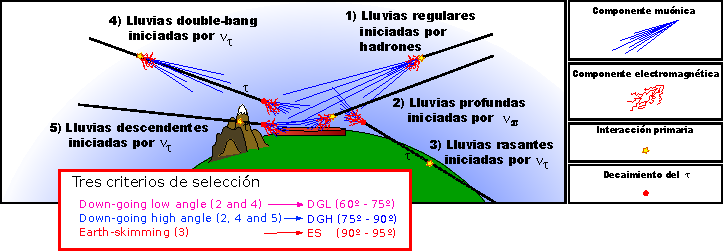
\includegraphics[width=\textwidth]{./fig/estrategiaAuger/auger_nu}
		% curveEarthSketch.png: 2404x1199 pixel, 150dpi, 40.70x20.30 cm, bb=0 0 1154 575
		\caption{\label{fig:augerNu}
		Posibles canales de detección de neutrinos en auger. Se detallan los tres análisis que fueron optimizados para identificar neutrinos provenientes de los diferentes canales.
		}
	\end{figure}
Debido a la diferencias esenciales que presentan estos canales de detección, en Auger existen actualmente tres búsquedas optimizadas para distintos rangos de ángulo zenital:
\begin{itemize}
 \item DGL: optimizado para buscar neutrinos down-going con ángulo entre $60^\circ$ y $75^\circ$.
 \item DGH: idem DGL pero para ángulos entre $75^\circ$ y $90^\circ$. 
 \item ES: optimizado para detectar neutrinos earth-skimming para ángulos entre $90^\circ$ y $95^\circ$.
\end{itemize}

En los tres casos, la estrategia utilizada para la búsqueda fue del tipo \emph{análisis ciego}, cuyo proceder se esquematizan en la figura \ref{fig:strAuger}.
	\begin{figure}[ht!]
		\centering
		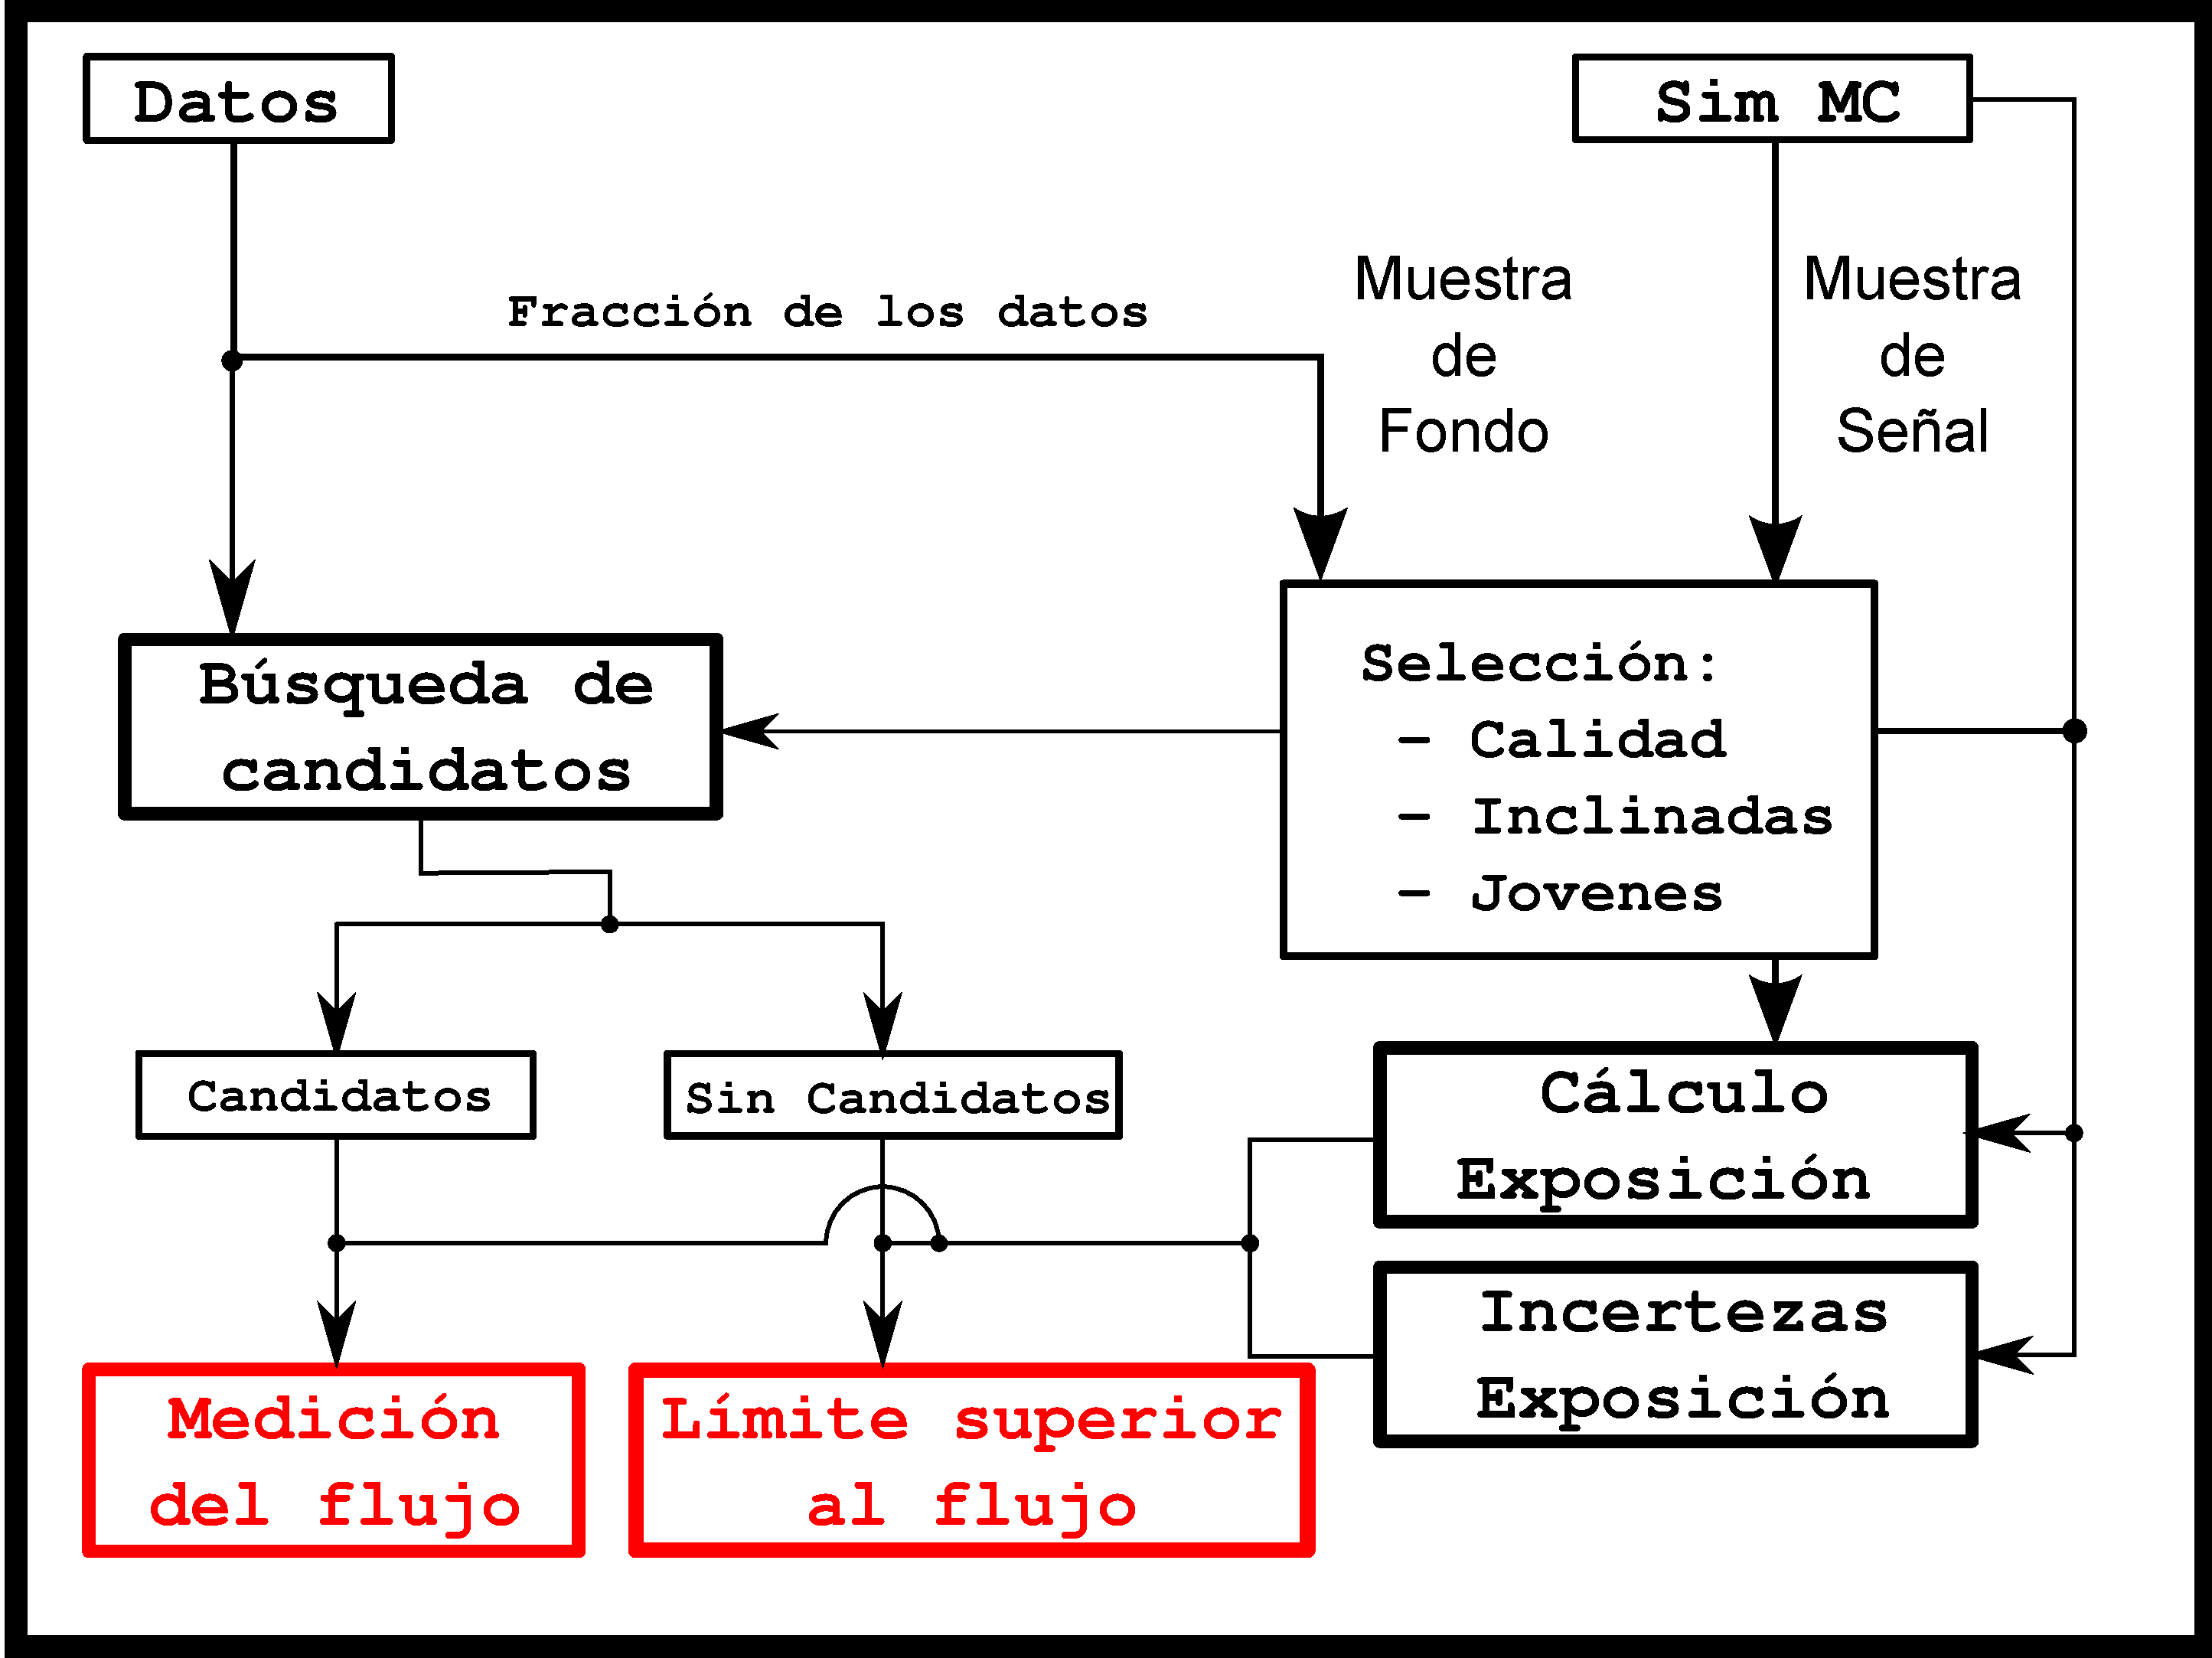
\includegraphics[width=\textwidth]{./fig/estrategiaAuger/analysisSchema}
		\caption{\label{fig:strAuger}
		Esquema de la estrategia utilizada en las búsquedas de neutrinos con el Observatorio Pierre Auger.
		}
	\end{figure}
Este consiste en definir un criterio de selección mediante el cual se decidirá si un evento es candidato a neutrino o no, sin utilizar datos o utilizando una pequeña fracción de los mismos que luego no podrá ser utilizada para la búsqueda.

Para definir este criterio es necesario contar con una muestra de señal y otra de fondo.
En los tres análisis se utilizaron simulaciones de Monte Carlo para generar una muestra de señal y una pequeña fracción de los datos ($\sim15\%$) como muestra de fondo, debido a que se encuentran completamente dominados por eventos que no son neutrinos.
Una vez definidas las muestras de señal y fondo, se eligieron criterios de calidad con el fin de eliminar eventos espureos y se optimizaron cortes en diferentes variables del detector que permiten elegir las lluvias jóvenes entre las inclinadas.
Así, con el criterio de selección listo es posible, por un lado calcular la exposición del detector a los distintos tipos de neutrinos y estimar las incertezas sistemáticas cometidas, y por el otro realizar la búsqueda de candidatos sobre los datos que no fueron utilizados hasta el momento.
Luego, si hubiese candidatos sería posible informar la magnitud de el flujo con su error, o en caso contrario ponerle una cota superior.

En los próximos capítulos se abordarán las distintas etapas de este análisis para las tres búsquedas.

% \textbf{DEBERIA MENCIONAR LAS TRES TESIS EN ESTA SECCION ME PARECE}
